% 1.5.28

\documentclass[a4paper, 11pt]{article}
\usepackage{multicol}
\usepackage{tabularx}
\usepackage{enumitem}
\usepackage[a5paper, margin=10mm, onecolumn]{geometry}
\usepackage{listings}
\usepackage{amssymb}
\usepackage{gvv}
\usepackage{gvv-book}
\usepackage{amsmath}
\usepackage{setspace}
\usepackage{caption}

\author{EE25BTECH11041-Naman Kumar }
\graphicspath{ {./figs/} }

\begin{document}
\begin{center}
    \huge{1.5.28}\\
    \large{EE25BTECH11041 - Naman Kumar}
\end{center}
Question:\\
$\Vec{P} (5, -3)$ and $\Vec{Q}$ (3, y) are the points of trisection of the line segment joining $\Vec{A} (7, -2)$ and $\Vec{B} (1, -5)$. Then y equals.

\solution \\
%\begin{align}
%\text{Distance of }\Vec{P} \text{ from A}: \sqrt{(7-5)^2 + (3-2)^2} =\sqrt{5}\\
%\text{Distance of }\Vec{P} \text{ from B}: \sqrt{(1-5)^2 + (5-3)^2} =\sqrt{20}
%\end{align}
%Ratio of equation of (1) and (2) = $\frac{1}{2}$\\
%therefore, $\Vec{Q}$ is nearer to $\Vec{B}$\\
\begin{align}
\Vec{Q}=\frac{1}{1+k}\brak{\Vec{A}+k\Vec{B}}\\
\end{align}
Putting values of k, $\Vec{A}$ and $\Vec{B}$\\
\begin{align}
\Vec{Q}=\frac{1}{1+\frac{2}{1}}\brak{\myvec{7\\-2}+2\myvec{1\\-5}}\\
\Vec{Q}=\frac{1}{1+\frac{2}{1}}\brak{\myvec{7\\-2}+\myvec{2\\-10}}\\
\Vec{Q}=\frac{1}{1+2}\brak{\myvec{9\\-12}}\\
\Vec{Q}=\myvec{3\\-4}\\
\Vec{Q}=\myvec{3\\y}=\myvec{3\\-4}
\end{align}
\begin{center}
Therefore, y=-4
\end{center}
\newpage
\begin{figure}
    \centering
    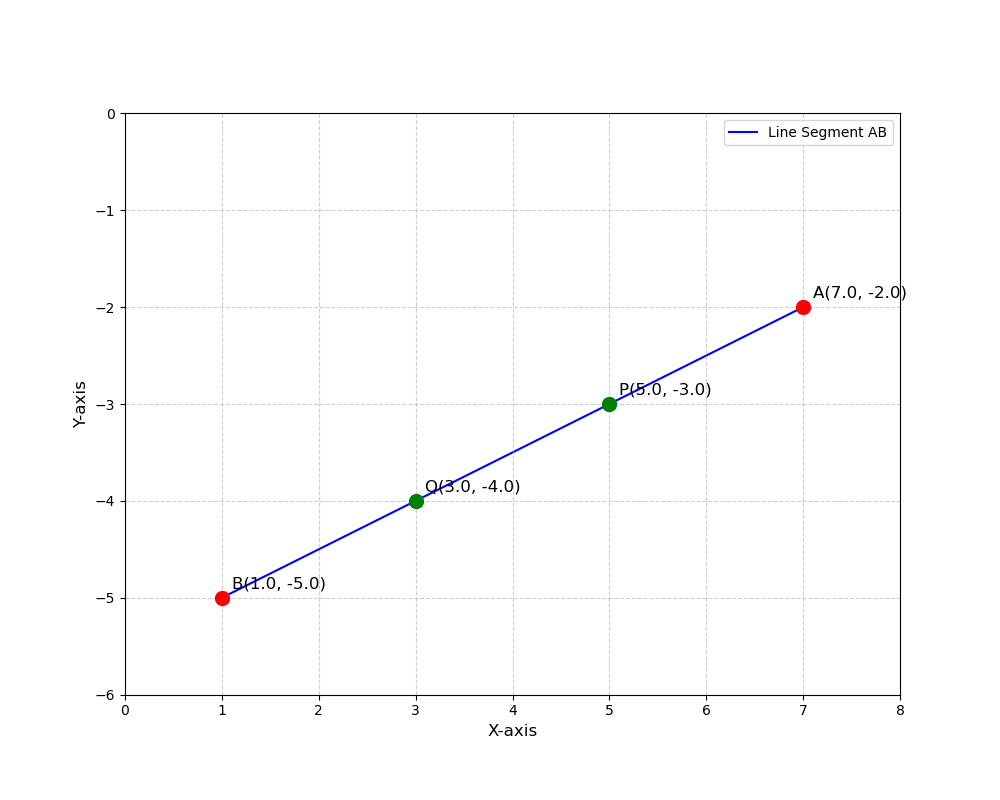
\includegraphics[width=\columnwidth]{figs/trisection_diagram.png}
    \caption{Caption}
    \label{fig:placeholder}
\end{figure}


\end{document}
